\documentclass[../../main.tex]{subfiles}

\graphicspath{{../../image/}{../../figure/}}

\begin{document}

\section{偏差-方差权衡}\label{section:ch04-偏差方差权衡}

到目前为止，在对回归问题的线性模型进行讨论时，我们假设基函数的形式和数量都是给定的（参见\cref{section:ch01-多项式拟合}）。我们还看到，如果使用非常有限的数据集训练复杂模型，使用最大似然估计可能会导致严重的过拟合问题。然而，通过限制基函数的数量来避免过拟合有一个副作用，就是限制了模型捕捉数据中有趣和重要趋势的灵活性。正则化项可以控制包含大量参数的模型的过拟合问题，但这又引出了如何确定合适的正则化系数$\lambda$的问题。我们可以从频率学派的视角讨论模型复杂性的问题，称为偏差-方差（bias-variance）权衡。

如果用参数向量$\boldsymbol{w}$控制的函数对$h(\boldsymbol{x})$进行建模，那么从贝叶斯学派的视角来看，模型中的不确定性可以通过$\boldsymbol{w}$上的后验分布来表示。但是频率学派会基于数据集$\mathcal{D}$对$\boldsymbol{w}$进行点估计，并试图通过思想实验来解释该估计的不确定性。假设我们有大量的数据集，每个数据集的大小为$N$且都独立地从分布$p(t\mid\boldsymbol{x})$中产生。对于任何给定的数据集$\mathcal{D}$，都可以通过算法得到预测函数$f(\boldsymbol{x};\mathcal{D})$。

在讨论回归问题的决策理论时（参见\cref{section:ch04-决策理论}），一旦知道条件分布$p(t\mid\boldsymbol{x})$，每个损失函数都会得到对应的最优预测。一个普遍的选择是平方损失函数，其最优预测由条件期望给出：

\begin{align}
  h(\boldsymbol{x})=\mathbb{E}[t\mid\boldsymbol{x}]=\int t\,p(t\mid\boldsymbol{x})\,\mathrm{d}t
  \label{align:ch04-回归函数h}
\end{align}

平方损失的期望可以写成

\begin{align}
  \mathbb{E}[L]=\int\{f(\boldsymbol{x})-h(\boldsymbol{x})\}^{2}p(\boldsymbol{x})\,\mathrm{d}\boldsymbol{x}+\iint\{h(\boldsymbol{x})-t\}^{2}p(\boldsymbol{x},t)\,\mathrm{d}\boldsymbol{x}\,\mathrm{d}t
  \label{align:ch04-期望损失分解}
\end{align}

右侧的第二项来自数据上的固有噪声，与$f(\boldsymbol{x})$无关，它代表了期望损失的最小值。右侧的第一项取决于如何选择函数$f(\boldsymbol{x})$，因为这一项是非负的，所以能达到的最小值是$0$。

式\eqref{align:ch04-期望损失分解}右侧第一项的被积函数，在一个特定的数据集$\mathcal{D}$上为$\{f(\boldsymbol{x};\mathcal{D})-h(\boldsymbol{x})\}^{2}$。由于它的值依赖于特定的数据集$\mathcal{D}$，我们取其在数据集上的期望。在花括号内加减$\mathbb{E}_{\mathcal{D}}[f(\boldsymbol{x};\mathcal{D})]$，然后展开，可以得到

\begin{align}
  \mathbb{E}_{\mathcal{D}}\bigl[\{f(\boldsymbol{x};\mathcal{D})-h(\boldsymbol{x})\}^{2}\bigr]
  =\left\{\mathbb{E}_{\mathcal{D}}[f(\boldsymbol{x};\mathcal{D})]-h(\boldsymbol{x})\right\}^{2}
  +\mathbb{E}_{\mathcal{D}}\bigl[\{f(\boldsymbol{x};\mathcal{D})-\mathbb{E}_{\mathcal{D}}[f(\boldsymbol{x};\mathcal{D})]\}^{2}\bigr]
  \label{align:ch04-偏差方差分解}
\end{align}

因此期望损失可以分解为三项之和：

\begin{align}
  \mathbb{E}[L]=\text{平方偏差}+\text{方差}+\text{噪声}
  \label{align:ch04-偏差方差噪声}
\end{align}

其中

\begin{align}
  \text{平方偏差}=\int\left\{\mathbb{E}_{\mathcal{D}}[f(\boldsymbol{x};\mathcal{D})]-h(\boldsymbol{x})\right\}^{2}p(\boldsymbol{x})\,\mathrm{d}\boldsymbol{x}
  \label{align:ch04-平方偏差}
\end{align}

\begin{align}
  \text{方差}=\int\mathbb{E}_{\mathcal{D}}\bigl[\{f(\boldsymbol{x};\mathcal{D})-\mathbb{E}_{\mathcal{D}}[f(\boldsymbol{x};\mathcal{D})]\}^{2}\bigr]p(\boldsymbol{x})\,\mathrm{d}\boldsymbol{x}
  \label{align:ch04-方差}
\end{align}

\begin{align}
  \text{噪声}=\iint\{h(\boldsymbol{x})-t\}^{2}p(\boldsymbol{x},t)\,\mathrm{d}\boldsymbol{x}\,\mathrm{d}t
  \label{align:ch04-不可约噪声}
\end{align}

第一项称为平方偏差，表示所有数据集上的平均预测与期望回归函数的差异程度。第二项称为方差，衡量函数$f(\boldsymbol{x};\mathcal{D})$对被选的特定数据集的敏感程度。

我们的目标是最小化期望损失，它已被分解为平方偏差项、方差项和常数噪声项的和。偏差和方差之间存在权衡：非常灵活的模型具有低偏差和高方差，而相对稳定的模型具有高偏差和低方差。具有最优预测能力的模型能够在偏差和方差之间达到最佳平衡。

我们可以用第~1~章介绍过的正弦数据集来说明。独立生成$L=100$个数据集，每个数据集包含$N=25$个数据点，数据点由正弦曲线$h(x)=\sin(2\pi x)$产生。对每个数据集拟合一个包含$M=24$个高斯基函数和一个常数偏置基函数的模型（共$25$个参数），通过最小化正则化误差函数得到预测函数。较小的$\lambda$值允许模型对每个单独数据集上的噪声进行微调，从而导致较大的方差；相反，较大的$\lambda$值会使权重参数向$0$靠近，从而导致较大的偏差。

\begin{figure}[ht]
  \centering
  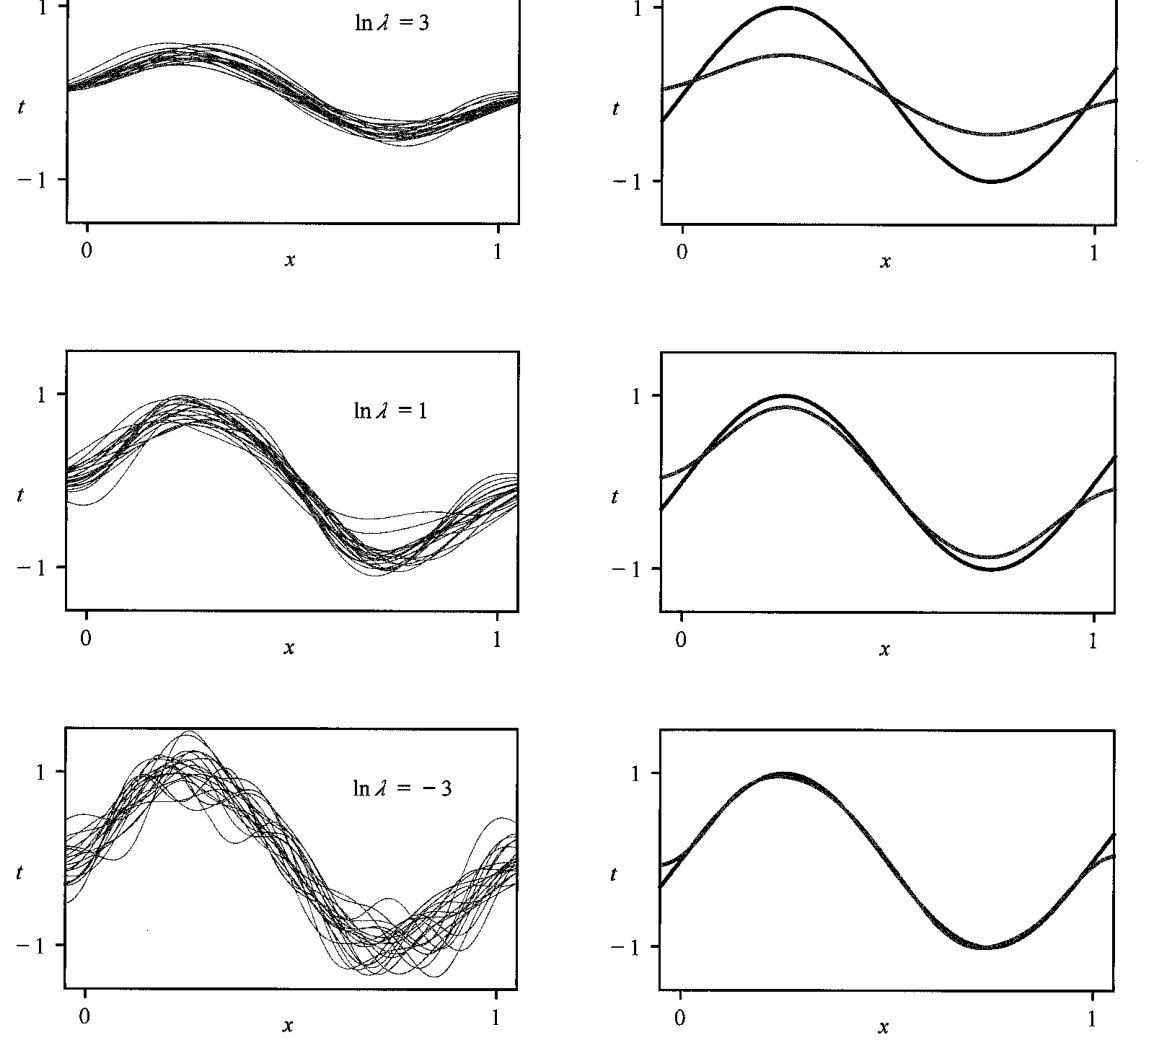
\includegraphics[width=0.7\textwidth]{ch04-fig4-7-bias-variance.png}
  \caption{使用正弦数据展示模型复杂度上偏差和方差的依赖关系，模型复杂度由正则化参数$\lambda$控制。$L=100$个数据集，每个含$N=25$个数据点，模型含$24$个高斯基函数及一个偏置基函数。左列：$100$次拟合中的$20$次随$\ln\lambda$变化的结果；右列：$100$次拟合的平均结果（粗曲线）与正弦目标函数（细曲线）。从上到下$\ln\lambda=3$（高偏差、低方差）、$\ln\lambda=1$（折中）、$\ln\lambda=-3$（低偏差、高方差）。}
  \label{figure:ch04-偏差方差示例}
\end{figure}

平均预测用下式估计：

\begin{align}
  \bar{f}(x)=\frac{1}{L}\sum_{l=1}^{L}f^{(l)}(x)
  \label{align:ch04-平均预测}
\end{align}

而平方偏差和方差则由下式给出：

\begin{align}
  \text{平方偏差}=\frac{1}{L}\sum_{l=1}^{L}\{\bar{f}(x)-h(x)\}^{2}
  \label{align:ch04-数值平方偏差}
\end{align}

\begin{align}
  \text{方差}=\frac{1}{L}\sum_{l=1}^{L}\{f^{(l)}(x)-\bar{f}(x)\}^{2}
  \label{align:ch04-数值方差}
\end{align}

偏差-方差分解的实际价值是有限的，因为它基于数据集集合的平均，而实际上我们只有单个观测数据集。如果有大量给定大小的独立训练集，更好的方法是将它们组合成单个更大的训练集，从而降低给定复杂度模型的过拟合风险。但尽管如此，偏差-方差分解仍经常提供对模型复杂性问题的有用洞察。

\end{document}
